\documentclass[
	% -- opções da classe memoir --
	12pt,				% tamanho da fonte
	openright,			% capítulos começam em pág ímpar (insere página vazia caso preciso)
	%twoside,			% para impressão em recto e verso. Oposto a oneside
	oneside,      % para impressão direta das páginas. Oposto a twoside
	a4paper,			% tamanho do papel.
	% -- opções da classe abntex2 --
	%chapter=TITLE,		% títulos de capítulos convertidos em letras maiúsculas
	%section=TITLE,		% títulos de seções convertidos em letras maiúsculas
	%subsection=TITLE,	% títulos de subseções convertidos em letras maiúsculas
	%subsubsection=TITLE,% títulos de subsubseções convertidos em letras maiúsculas
	% -- opções do pacote babel --
	english,			% idioma adicional para hifenização
	french,				% idioma adicional para hifenização
	spanish,			% idioma adicional para hifenização
	brazil,				% o último idioma é o principal do documento
	]{abntex2}\usepackage[]{graphicx}\usepackage[]{xcolor}
% maxwidth is the original width if it is less than linewidth
% otherwise use linewidth (to make sure the graphics do not exceed the margin)
\makeatletter
\def\maxwidth{ %
  \ifdim\Gin@nat@width>\linewidth
    \linewidth
  \else
    \Gin@nat@width
  \fi
}
\makeatother

\definecolor{fgcolor}{rgb}{0.345, 0.345, 0.345}
\newcommand{\hlnum}[1]{\textcolor[rgb]{0.686,0.059,0.569}{#1}}%
\newcommand{\hlstr}[1]{\textcolor[rgb]{0.192,0.494,0.8}{#1}}%
\newcommand{\hlcom}[1]{\textcolor[rgb]{0.678,0.584,0.686}{\textit{#1}}}%
\newcommand{\hlopt}[1]{\textcolor[rgb]{0,0,0}{#1}}%
\newcommand{\hlstd}[1]{\textcolor[rgb]{0.345,0.345,0.345}{#1}}%
\newcommand{\hlkwa}[1]{\textcolor[rgb]{0.161,0.373,0.58}{\textbf{#1}}}%
\newcommand{\hlkwb}[1]{\textcolor[rgb]{0.69,0.353,0.396}{#1}}%
\newcommand{\hlkwc}[1]{\textcolor[rgb]{0.333,0.667,0.333}{#1}}%
\newcommand{\hlkwd}[1]{\textcolor[rgb]{0.737,0.353,0.396}{\textbf{#1}}}%
\let\hlipl\hlkwb

\usepackage{framed}
\makeatletter
\newenvironment{kframe}{%
 \def\at@end@of@kframe{}%
 \ifinner\ifhmode%
  \def\at@end@of@kframe{\end{minipage}}%
  \begin{minipage}{\columnwidth}%
 \fi\fi%
 \def\FrameCommand##1{\hskip\@totalleftmargin \hskip-\fboxsep
 \colorbox{shadecolor}{##1}\hskip-\fboxsep
     % There is no \\@totalrightmargin, so:
     \hskip-\linewidth \hskip-\@totalleftmargin \hskip\columnwidth}%
 \MakeFramed {\advance\hsize-\width
   \@totalleftmargin\z@ \linewidth\hsize
   \@setminipage}}%
 {\par\unskip\endMakeFramed%
 \at@end@of@kframe}
\makeatother

\definecolor{shadecolor}{rgb}{.97, .97, .97}
\definecolor{messagecolor}{rgb}{0, 0, 0}
\definecolor{warningcolor}{rgb}{1, 0, 1}
\definecolor{errorcolor}{rgb}{1, 0, 0}
\newenvironment{knitrout}{}{} % an empty environment to be redefined in TeX

\usepackage{alltt}

% ---
% PACOTES
% ---

% ---
% Pacotes fundamentais
% ---
\usepackage{lmodern}			% Usa a fonte Latin Modern
\usepackage[T1]{fontenc}		% Selecao de codigos de fonte.
\usepackage[utf8]{inputenc}		% Codificacao do documento (conversão automática dos acentos)
\usepackage{indentfirst}		% Indenta o primeiro parágrafo de cada seção.
\usepackage{color}				% Controle das cores
\usepackage{graphicx}			% Inclusão de gráficos
\usepackage{microtype} 			% para melhorias de justificação
% ---

% ---
% Pacotes adicionais, usados apenas no âmbito do Modelo Canônico do abnteX2
% ---
\usepackage{lipsum}				% para geração de dummy text
% ---

% ---
% Pacotes de citações
% ---
\usepackage[brazilian,hyperpageref]{backref}	 % Paginas com as citações na bibl
\usepackage[alf]{abntex2cite}	% Citações padrão ABNT

% ---
% CONFIGURAÇÕES DE PACOTES
% ---

% ---
% Configurações do pacote backref
% Usado sem a opção hyperpageref de backref
\renewcommand{\backrefpagesname}{Citado na(s) página(s):~}
% Texto padrão antes do número das páginas
\renewcommand{\backref}{}
% Define os textos da citação
\renewcommand*{\backrefalt}[4]{
	\ifcase #1 %
		Nenhuma citação no texto.%
	\or
		Citado na página #2.%
	\else
		Citado #1 vezes nas páginas #2.%
	\fi}%
% ---

% ---
% Informações de dados para CAPA e FOLHA DE ROSTO
% ---
\titulo{Modelo de Regressão Logística Aplicada a Previsão de Inadimplência sobre Cartão de Crédito de uma Instituição Financeira}
\autor{DOUGLAS VINÍCIUS GONÇALVES ARAÚJO}
\local{JI-PARANÁ}
\data{2022}
\instituicao{%
  UNIVERSIDADE FEDERAL DE RONDÔNIA -- UNIR
  \par
  DEPARTAMENTO DE MATEMÁTICA E ESTATÍSTICA
  \par
  RELATÓRIO DE PESQUISA}
\tipotrabalho{Tese (Doutorado)}
% O preambulo deve conter o tipo do trabalho, o objetivo,
% o nome da instituição e a área de concentração
\preambulo{Relatório de Estágio Supervisionado apresentado como Trabalho de Pesquisa à Coordenação do Curso de Bacharelado em Estatística da Universidade Federal de Rondônia.}
% ---

% ---
% Configurações de aparência do PDF final

% alterando o aspecto da cor azul
\definecolor{blue}{RGB}{41,5,195}

% informações do PDF
\makeatletter
\hypersetup{
     	%pagebackref=true,
		pdftitle={\@title},
		pdfauthor={\@author},
    	pdfsubject={\imprimirpreambulo},
	    pdfcreator={LaTeX with abnTeX2},
		pdfkeywords={abnt}{latex}{abntex}{abntex2}{projeto de pesquisa},
		colorlinks=true,       		% false: boxed links; true: colored links
    	linkcolor=blue,          	% color of internal links
    	citecolor=blue,        		% color of links to bibliography
    	filecolor=magenta,      		% color of file links
		urlcolor=blue,
		bookmarksdepth=4
}
\makeatother
% ---

% ---
% Espaçamentos entre linhas e parágrafos
% ---

% O tamanho do parágrafo é dado por:
\setlength{\parindent}{1.3cm}

% Controle do espaçamento entre um parágrafo e outro:
\setlength{\parskip}{0.2cm}  % tente também \onelineskip

% ---
% compila o indice
% ---
\makeindex
% ---

% ----
% Início do documento
% ----
\IfFileExists{upquote.sty}{\usepackage{upquote}}{}
\begin{document}

% Seleciona o idioma do documento (conforme pacotes do babel)
%\selectlanguage{english}
\selectlanguage{brazil}

% Retira espaço extra obsoleto entre as frases.
\frenchspacing

% ----------------------------------------------------------
% ELEMENTOS PRÉ-TEXTUAIS
% ----------------------------------------------------------
% \pretextual

% ---
% Capa
% ---
\imprimircapa
% ---

% ---
% Folha de rosto
% ---
\imprimirfolhaderosto
% ---
\clearpage
% ---
% NOTA DA ABNT NBR 15287:2011, p. 4:
%  ``Se exigido pela entidade, apresentar os dados curriculares do autor em
%     folha ou página distinta após a folha de rosto.''
% ---
\begin{agradecimentos} 
  Os agradecimentos... 
\end{agradecimentos}
% ---
% Epígrafe

\begin{epigrafe} 
  \vspace*{\fill} 
  \begin{flushright} 
  \textit{"Os livros servem para nos lembrar quanto somos estúpidos e tolos. 
      \\ São o guarda pretoriano de César, cochichando enquanto o desfile ruge 
      \\ pela avenida: – Lembre-se, César, tu és mortal. A maioria de nós não 
      \\ pode sair correndo por aí, falar com todo mundo, conhecer todas as 
      \\ cidades do mundo, não temos tempo, dinheiro ou tantos amigos assim. 
      \\ As coisas que você está procurando, Montag, estão no mundo, mas a 
      \\ única possibilidade que o sujeito comum terá de ver noventa e nove 
      \\ por cento delas está num livro". 
      \\ - Fahrenheit 451 de Ray Douglas Bradbury} 
  \end{flushright} 
\end{epigrafe}
% ---

% --- resumo em português--
\begin{resumo} 
  O objetivo deste trabalho é aplicar o modelo de regressão logística a dados
  de cartão de crédito de uma instituição financeira do estado de Rondônia.
  \vspace{\onelineskip} 
  \noindent
  
  \textbf{Palavras-chaves}: Risco de Crédito, Probabilidade de Default, Modelo de Regressão Logístico. 
\end{resumo}

% ---
% inserir lista de ilustrações
% ---
\pdfbookmark[0]{\listfigurename}{lof}
\listoffigures*
\cleardoublepage
% ---

% ---
% inserir lista de tabelas
% ---
\pdfbookmark[0]{\listtablename}{lot}
\listoftables*
\cleardoublepage
% ---

% ---
% inserir lista de abreviaturas e siglas
% ---
\begin{siglas}
  \item[ABNT] Associação Brasileira de Normas Técnicas
  \item[abnTeX] ABsurdas Normas para TeX
\end{siglas}
% ---

% ---
% inserir lista de símbolos
% ---
\begin{simbolos}
  \item[$ \Gamma $] Letra grega Gama
  \item[$ \Lambda $] Lambda
  \item[$ \zeta $] Letra grega minúscula zeta
  \item[$ f(x;\theta)$] Função de Densidade de Probabilidade
  \item[$ \Pi $] Produtório
\end{simbolos}
% ---

% ---
% inserir o sumario
% ---
\pdfbookmark[0]{\contentsname}{toc}
\tableofcontents*
\cleardoublepage
% ---

% ----------------------------------------------------------
% ELEMENTOS TEXTUAIS
% ----------------------------------------------------------
\textual

% ----------------------------------------------------------
% Introdução
% ----------------------------------------------------------
\chapter[Introdução]{Introdução}
%\addcontentsline{toc}{chapter}{INTRODUÇÃO}



  \section{Objetivos}

O objetivo deste trabalho é desenvolver um modelo de previsão de risco de inadimplência 
dos tomadores de cartões de créditos de uma instituição Financeira do Estado de Rondônia.






% ----------------------------------------------------------
% Capitulo de textual
% ----------------------------------------------------------
\chapter{REFERENCIAL TEÓRICO}


  \section{Credit Scoring}
  
  
  
  
  \section{Breve Introdução sobre Machine Learning}
  
Uma definição básica sobre Machine Learning (Aprendizado de Máquina) é englobar 
um conjunto de regras com algoritmos e procedimentos que tem como objetivo de 
extrair informações apartir dos dados e dessas informações tomar uma decisão.

Segundo \cite{goodfellow2016deep}, os algoritmos de Machine Learning podem ser 
amplamente categorizados como aprendizados Supervisionado e Não-Supervisionados, 
sitentizando essa diferença, é o tipo de experiência durante o aprendizado do 
algoritmo.

  
    \begin{figure}
      \caption{\label{img1}Machine Learning e suas aplicações}
      \begin{center}
        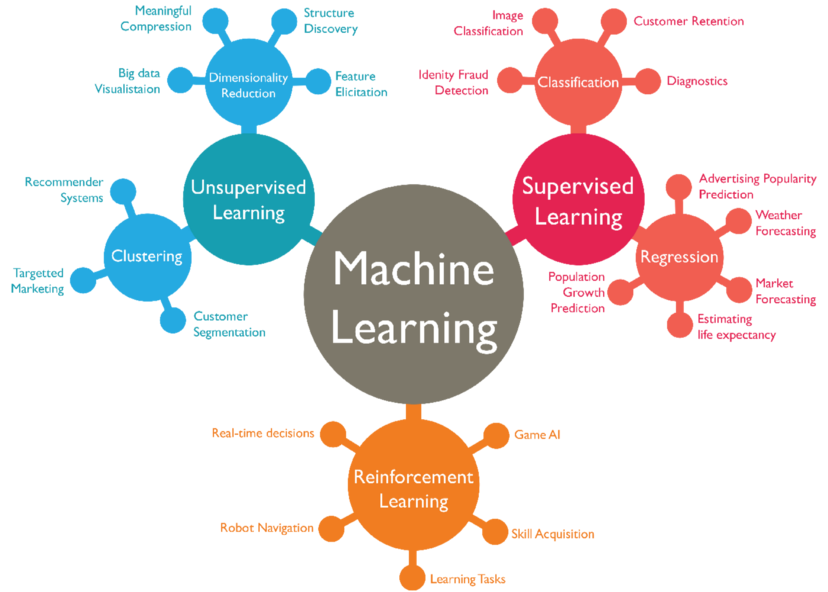
\includegraphics[scale = 0.4]{image/img1.png}
      \end{center}
      \legend{Fonte: https://becominghuman.ai/an-introduction-to-machine-learning}
    \end{figure}
  
  \section{Modelo de Regressão Logística}
  
A regressão logística tem como principal uso modelar uma variável binária $(0,1)$,
com base em mais variáveis, estas chamadas de variáveis explicativas ou preditoras.
E comumentemente a variável resposta ou dependente, assim chama-se a variável
binária do modelo. Conforme \cite{hilbe2016practical}, o melhor modelo ajustado 
aos dados é assumido que:
\begin{itemize}
  \item Não há correlação entre as variáveis preditoras;
  \item Estejam significativamente relacionados com a resposta;
  \item Que as observações dos dados não estejam correlacionados com a resposta.
\end{itemize}
  
A resposta do modelo dito está conveniente a uma distribuição subjacente, ou seja,
segue uma distribuição de Bernoulli. Como esta distribuição é um subconjunto da distribuição 
Binomial que a função de probabilidade pode ser expressa:
\begin{equation}
  f(x;\theta) = \prod_{i = 1}^{n}\theta_{i}^{x_i}(1 - \theta_{i})^{1 - x_i}
\end{equation}





      \subsection{Interpretação dos Paramêtros}




      \subsection{Estimação dos Paramêntros}





      \subsection{Testes de Significância}





      \subsection{Seleção de Variáveis}




      \subsection{Desempenho dos Modelos}


\chapter{Metodologia e Dados}






\chapter{Resultados e Discussões}





\chapter{Considerações Finais}




% ----------------------------------------------------------
\bibliography{abntex2-modelo-references}

% ----------------------------------------------------------
% Glossário
% ----------------------------------------------------------
%
% Consulte o manual da classe abntex2 para orientações sobre o glossário.
%
%\glossary


% ----------------------------------------------------------
% Apêndices
% ----------------------------------------------------------

% ---
% Inicia os apêndices
% ---
\begin{apendicesenv}

% Imprime uma página indicando o início dos apêndices
\partapendices

% ----------------------------------------------------------
\chapter{DESCRIÇÃO DAS VARIÁVEIS}
% ----------------------------------------------------------

\begin{tabular}{ccc} 
  \hline 
  Coluna 1 & Coluna 2 & Coluna 3 \\ 
  \hline 
  Coluna 1 Coluna 2 Coluna 3 A B D E C F A & B & C \\
  D & E & F \\ 
  \hline 
\end{tabular}


% ----------------------------------------------------------
\chapter{SCRIPT R}
% ----------------------------------------------------------



\end{apendicesenv}
% ---

\begin{comment}
% ----------------------------------------------------------
% Anexos
% ----------------------------------------------------------

% ---
% Inicia os anexos
% ---
\begin{anexosenv}

% Imprime uma página indicando o início dos anexos
\partanexos

% ---
\chapter{Morbi ultrices rutrum lorem.}
% ---
\lipsum[30]

% ---
\chapter{Cras non urna sed feugiat cum sociis natoque penatibus et magnis dis
parturient montes nascetur ridiculus mus}
% ---

\lipsum[31]

% ---
\chapter{Fusce facilisis lacinia dui}
% ---

\lipsum[32]

\end{anexosenv}
\end{comment}
%---------------------------------------------------------------------
% INDICE REMISSIVO
%---------------------------------------------------------------------

\phantompart

\printindex



\end{document}
